\documentclass[11pt]{article}
\usepackage{graphicx}
\usepackage{placeins}


% acronyms for text or math mode
\newcommand {\ccast} {\mbox{\small CCAST}}
\newcommand {\cris} {\mbox{\small CrIS}}

\newcommand {\airs} {\mbox{\small AIRS}}
\newcommand {\iasi} {\mbox{\small IASI}}
\newcommand {\idps} {\mbox{\small IDPS}}
\newcommand {\nasa} {\mbox{\small NASA}}
\newcommand {\noaa} {\mbox{\small NOAA}}
\newcommand {\nstar} {\mbox{\small STAR}}
\newcommand {\umbc} {\mbox{\small UMBC}}
\newcommand {\uw}   {\mbox{\small UW}}

\newcommand {\fft}  {\mbox{\small FFT}}
\newcommand {\ifft} {\mbox{\small IFFT}}
\newcommand {\fir}  {\mbox{\small FIR}}
\newcommand {\fov}  {\mbox{\small FOV}}
\newcommand {\for}  {\mbox{\small FOR}}
\newcommand {\ict}  {\mbox{\small ICT}}
\newcommand {\ils}  {\mbox{\small ILS}}
\newcommand {\igm}  {\mbox{\small IGM}}
\newcommand {\opd}  {\mbox{\small OPD}}
\newcommand {\rms}  {\mbox{\small RMS}}
\newcommand {\zpd}  {\mbox{\small ZPD}}
\newcommand {\ppm}  {\mbox{\small PPM}}
\newcommand {\srf}  {\mbox{\small SRF}}
\newcommand {\sdr}  {\mbox{\small SDR}}

\newcommand {\ES} {\mbox{\small ES}}
\newcommand {\SP} {\mbox{\small SP}}
\newcommand {\IT} {\mbox{\small IT}}
\newcommand {\SA} {\mbox{\small SA}}

\newcommand {\ET} {\mbox{\small ET}}
\newcommand {\FT} {\mbox{\small FT}}

\newcommand {\wn} {\mbox{cm$^{-1}$}}

% abbreviations, mainly for math mode
\newcommand {\real} {\mbox{real}}
\newcommand {\imag} {\mbox{imag}}
\newcommand {\atan} {\mbox{atan}}
\newcommand {\obs}  {\mbox{obs}}
\newcommand {\calc} {\mbox{calc}}
\newcommand {\sinc} {\mbox{sinc}}
\newcommand {\psinc} {\mbox{psinc}}
\newcommand {\std} {\mbox{std}}

% symbols, for math mode only
\newcommand {\lmax} {L_{\mbox{\tiny max}}}
\newcommand {\vmax} {V_{\mbox{\tiny max}}}

\newcommand {\tauobs} {\tau_{\mbox{\tiny obs}}}
\newcommand {\taucal} {\tau_{\mbox{\tiny calc}}}
\newcommand {\Vdc}  {V_{\mbox{\tiny DC}}}

\newcommand {\rIT} {r_{\mbox{\tiny\textsc{ict}}}}
\newcommand {\rES} {r_{\mbox{\tiny\textsc{es}}}}
\newcommand {\robs} {r_{\mbox{\tiny obs}}}

\newcommand {\rITobs} {r_{\mbox{\tiny\textsc{ict}}}^{\mbox{\tiny obs}}}
\newcommand {\rITcal} {r_{\mbox{\tiny\textsc{ict}}}^{\mbox{\tiny cal}}}

\newcommand {\ITmean} {\langle\mbox{\small IT}\rangle}
\newcommand {\SPmean} {\langle\mbox{\small SP}\rangle}


\title{AIRS Deconvolution and Translation \\
  from the AIRS to CrIS IR Sounders \\
  \vspace{3mm}
  {****} DRAFT {****}\\
}

\author{Howard E.~Motteler \\
  L.~Larrabee Strow \\
  \\
  UMBC Atmospheric Spectroscopy Lab \\
  Joint Center for Earth Systems Technology \\
}

\date{\today}
\begin{document}
\maketitle

\section{Introduction}

Upwelling infrared radiation as measured by the {\airs} \cite{airs1}
and {\cris} \cite{cris1,cris2} sounders is a significant part of the
long term climate record.  We would like to treat this as a single
data set and often want to compare radiances, for example in the
analysis of simultaneous nadir overpasses (SNOs) for sounder
calibration or validation.  However the instruments have different
spectral resolutions, channel response functions, and band spans.
As a step in addressing this problem we consider the translation of
channel radiances from {\airs} to standard resolution {\cris}.

Translation from {\airs} to {\cris} involves more that basic
resampling.  {\airs} is a grating spectrometer with a distinct
response function for each channel determined by the focal plane
geometery, while {\cris} is a Michaelson interferometer with a sinc
response function, after calibration and corrections.  In section
\ref{decon} we show how to take advantage of our detailed knowledge
of the {\airs} spectral response functions (SRFs) and their overlap
to deconvolve channel radiances to a resolution-enhanced
intermediate representation, typically a $0.1$~\wn\ grid, the
approximate resolution of the tabulated {\airs} SRFs.  This can be
reconvolved to an idealized grating instrument, and the resolving
power of the reconvolution measured.

Similarly, the {\airs} to {\cris} translation consists of two steps,
deconvolution of the {\airs} channel radiances to the intermediate
grid, followed by reconvolution to the {\cris} user grid.  Section
\ref{airs2cris} gives the details and validation tests.  In section
\ref{statfix} we show how to further improve residuals by adding a
statistically based correction.  Section \ref{appcon} gives some
applications and conclusions.

\FloatBarrier
\section{AIRS Deconvolution}
\label{decon}

The {\airs} spectral response functions model channel response as a
function of frequency and associate channels with nominal center
frequencies.  Each {\airs} channel $i$ has an associated spectral
response function or {\srf} $\sigma_i(v)$ such that the channel
radiance $c_i = \int \sigma_i(v)r(v)\,dv$, where $r$ is radiance at
frequency $v$.  The center or peak of $\sigma_i$ is the nominal
channel frequency.

\begin{figure} % source plot_SRF2.m
  \centering
  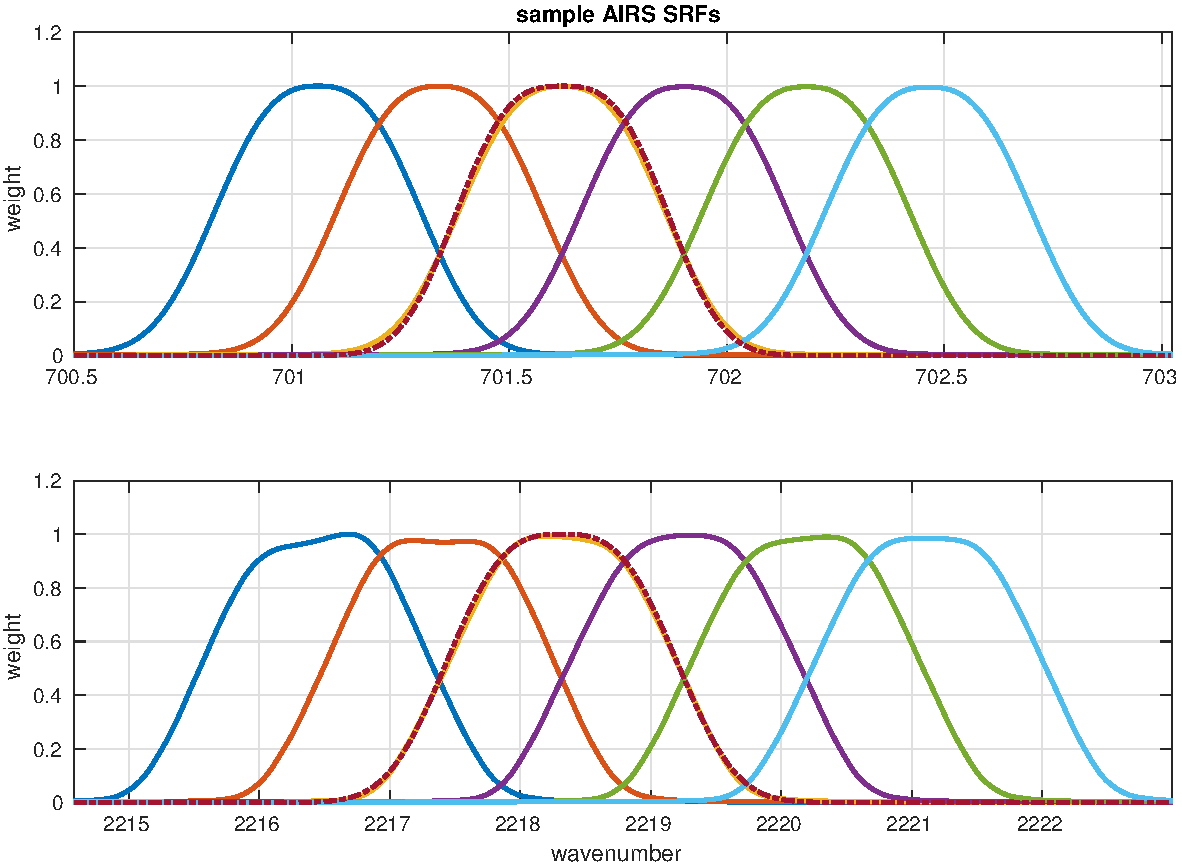
\includegraphics[height=7.5cm]{figures/airs_sample_srfs.pdf}
  \caption{sample {\airs} spectral response functions from the low
    and high ends of the band.   The dashed line is a generalized
    Gaussian function.}
  \label{srfs1}
\end{figure}

\begin{figure} % source plot_SRF2.m
  \centering
  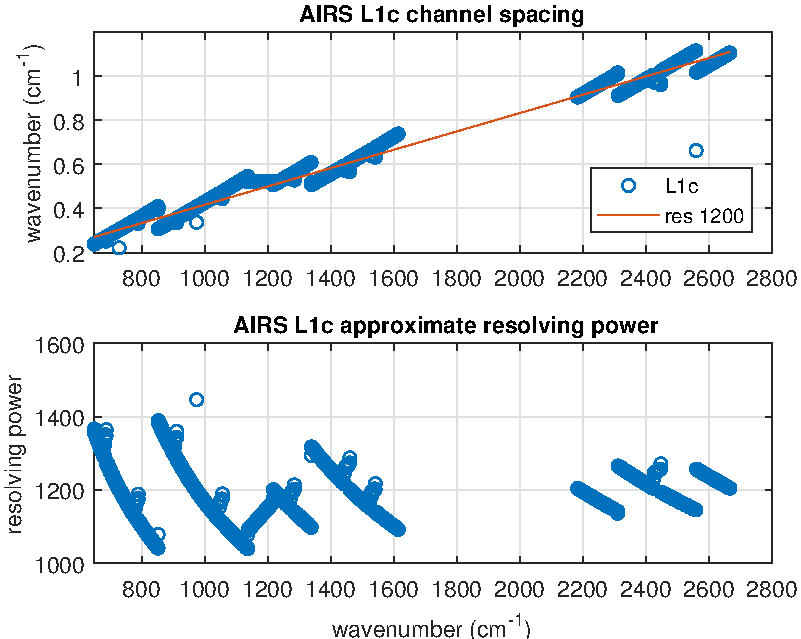
\includegraphics[height=7.5cm]{figures/airs_L1c_res.pdf}
  \caption{{\airs} L1c channel spacing and derived resolving
    power}
  \label{chan1}
\end{figure}

\begin{figure} % source plot_Binv.m
  \centering
  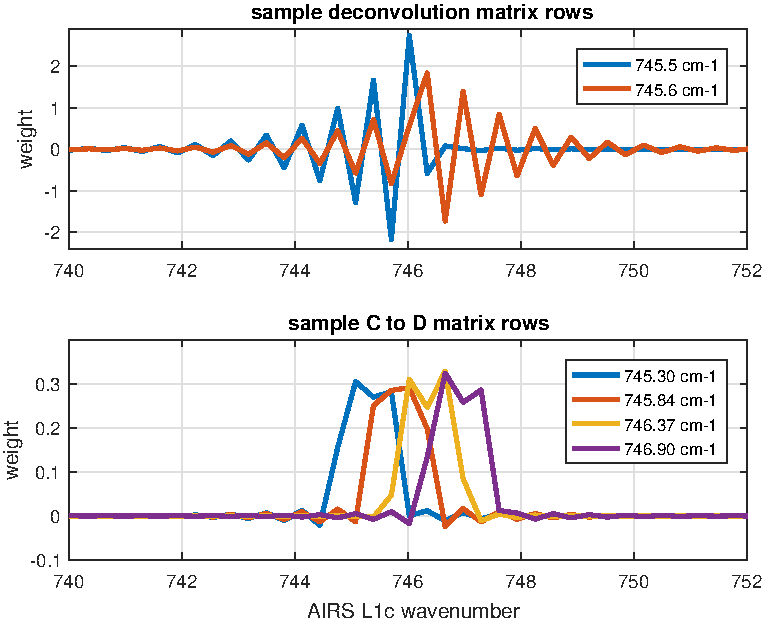
\includegraphics[height=7.5cm]{figures/airs_decon_basis.pdf}
  \caption{sample adjacent basis functions for the deconvolved
    {\airs} radiances}
  \label{dbasis}
\end{figure}

Figure \ref{srfs1} shows typical {\airs} SRFs from the low and high
ends of the band.  Note the significant overlap in the wings.  This
allows the deconvolution to recover resolution beyond that of the
response functions considered individually.  The SRFs are not
necessarily symmetrical, especially at the high end of the band.
The dashed line is a 1-parameter fit of a generalized Gaussian,
which we consider in more detail later in this section.  Figure
\ref{chan1} shows channel spacing and resolving power for the
{\airs} L1c channel set \cite{airs1c}.  The variable channel spacing
and resolving power are due to the modular structure of the focal
plane.  Although not entirely regular---that is, not a simple
function of frequency---the L1c channel set is more regular than the
L1b channel set from which it is derived, and we mainly consider the
L1c set here.

Suppose we have $n$ channels and a frequency grid $\vec v$ of $k$
points spanning the union of the domains of the functions
$\sigma_i$.  The grid step size for our applications is often 0.0025
{\wn}, the kcarta resolution \cite{kcarta1}.  Let $S_k$ be an
$n\times k$ array such that $s_{i,j} = \sigma_i(v_j)/w_i$, where
$w_i = \sum_j \sigma_i(v_j)$, that is where row $i$ is $\sigma_i(v)$
tabulated at the grid $\vec v$ and normalized so the row sum is 1.
If the channel centers are in increasing order $S_k$ is banded, and
if they are not too close (as is the case for a few of the L1b
channels) the rows are linearly independent.  $S_k$ is a linear
transform whose domain is radiance at the grid $\vec v$ and whose
range is channel radiances.  If $r$ is radiance at the grid $\vec
v$, then $c = S_k r$ gives a good approximation of the channel
radiances $c_i = \int\sigma_i(v)r(v)\,dv$.

In practice this is how we convolve kcarta or other simulated
radiances to get {\airs} channel radiances, for example to get
reference truth for the tests shown here.  We construct $S_k$ either
explicitly or implicitly from the {\airs} {\srf} tabulations.  The
matrix $S_k$ in the former case is large but manageable with a
banded or sparse representation.

Suppose we have $S_k$ and channel radiances $c$ and want to find
$r$, that is, to deconvolve $c$.  Consider the linear system $S_k x
= c$.  Since $n < k$ for the kcarta grid mentioned above this is
underdetermined, with infinitely many solutions.  To solve this
system we could add constraints, take a pseudo-inverse, consider a
new matrix $S_b$ with columns tabulated at some coarser grid, or
some combination of the above.

For the {\airs} to {\cris} translation we are mainly interested in 
the transform $S_b$ for {\srf}s at an intermediate grid, typically
0.1 {\wn}, the approximate resolution of the {\srf} measurements.
Let $\vec v_b = v_1,v_2,\ldots,v_m$ be a 0.1 {\wn} grid spanning the
domains of the functions $\sigma_i$.  Similar to $S_k$, let $S_b$ be
an $n\times m$ array where row $i$ is $\sigma_i(v)$ tabulated at the
$\vec v_b$ grid, with rows normalized to~1.  If $r$ is radiance at
the $\vec v_b$ grid, then $c = S_b r$ is still a reasonable
approximation of $\int\sigma_i(v)r(v)\,dv$.

Consider the linear system $S_b x = c$, similar to the case $S_k x =
c$ above, where we are given $S_b$ and channel signals $c$ and want
to find radiances $x$.  Since $n < m < k$, as with $S_k$ the system
will be underdetermined, but more manageable because $m$ is
approximately 40 times less than $k$.  After some preliminary tests
we settled on a Moore-Penrose pseudoinverse for $S_b^{-1}$.  Then $x
= S_b^{-1} c$ gives us deconvolved radiances at the {\srf} tabulation
grid.  Figure \ref{dbasis} shows adjacent typical basis function for
the deconvolution, that is, adjacent columns of the pseudo-inverse
$S_b^{-1}$.  The functions are vaugely sinc-like, though the negative
excursions are significantly greater.  For each channel $c$, the
associated column values show the span of influence of $c$ in the
deconvolution.

The {\airs} deconvolution gives a significant resolution enhancement,
though at the cost of added artifacts and noise.  Figure \ref{dspec}
shows spectra for a simulated deconvolution together with the direct
convolution of kcarta 0.0025~\wn\ radiances to the 0.1~{\wn}
intermediate grid, for fitting profile 1.  Figure \ref{ddiff} shows
the mean and standard deviation of the difference of the deconvolved
minus the directly convolved radiances for all 49 fitting profiles
\cite{sarta1,sarta2}.  Note that convolution, deconvolution, and
apodization are done with radiances while spectra are presented and
statistics done after translation to brightness temperatures.
The residuals are large and mainly significant for understanding
limitations of the deconvolution.  We do not propose using the
deconvolved radiances directly; they are an intermediate step for
reconvolution to a lower resolution grating instrument as described
below or to the {\cris} user grid as described in the next section.

The deconvolution is done by first convolving kcarta radiances to the
{\airs} L1c channel set to get ``true {\airs}'' and then deconvolving
this to the 0.1~\wn\ grid, as discussed above.  The direct
convolution is for a hypothetical grating spectrometer with a
resolving power of 2000, oversampled to the 0.1~\wn\ grid.  The
choice of basis functions for reference truth for the intermediate
0.1~\wn\ grid is not obvious, since the deconvolution is undoing---at
least to some extent---the effects of the {\airs} SRF convolutions.
The response function we used for this, and for the ``L1d basis''
discussed below, is a generalized Gaussian of the form
\[w = \exp\left(-\left(\frac{(x - v_0)^2}{2c^2}\right)^{1.5}\right) \]
where $c=\fwhm / 2.355$ and $v_0$ is the desired channel center.  The
exponent $1.5$ is chosen to give an approximate match to {\airs} SRFs
with the same \fwhm, though without the fine structure and variation
of the latter.  Figure \ref{srfs1} shows two such functions paired
with {\airs} SRFs with the same \fwhm.

% We also tried the generalized Gaussian with a fixed \fwhm\ for
% values $0.4$, $0.6$, and $0.8$ and a sinc basis with a spacing of
% $0.2$~\wn, all of which gave larger residuals.  The residual was
% roughly minimized for the resolving power of 2000 shown here.

The residuals can be reduced dramatically by reconvolving the
$0.1$~\wn\ intermediate grid to the channel grid for an idealized
grating instrument with reduced resolving power.  Define an L1d basis
with the generalized Gaussian response function above, $\fwhm = v /
\hbox{resolving power}$, and $dv = \fwhm / 2$ with the $dv$-spaced
channel steps starting at $v_0$.  Note this is not oversampled, in
contrast with the regular spacing used for the 0.1~\wn\ intermediate
grid.

Figure \ref{L1d1200} shows residuals for reconvolution to such an L1d
basis with resolving power of 1200, the nominal {\airs} resolution.
For this and similar comparisons both the reference truth (``true
L1d'') and the reconvolution (L1c to L1d) are done to L1d channel
sets with the same resolving power and starting channel.  An L1d set
with a resolving power of 1200 gives a significant improvement over
the residual for the intermediate grid resolving power of 2000.
Figure \ref{L1d700s} shows residuals for a resolving power of 700.
This is less than the the residual for unapodized {\cris} shown in
section \ref{airs2cris} that we use as the starting point for our
{\airs} to {\cris} translations.  This is only half the best {\airs}
resolving power of 1400 in the LW.  Resolution is lost in shifting
channel centers to a single regular function of frequency.  The L1d
residuals dependend in part on the starting channel, and so on how
the SRF peaks line up and match with the L1c set.  The residuals
above are the result of a rough fit for $v_0$.  For a resolving power
of 1200 this is the first L1c channel, while for 700 it was the first
channel plus $0.2$~\wn.

The L1c to L1d translation can be represented as a single linear
transform $S_d\cdot S_c^{-1}$, where $S_c$ and $S_d$ are the
transform taking the intermediate grid to L1c and L1d channels and
$S_c^{-1}$ the pseudo-inverse of $S_c$, that is, the deconvolution
transform.  We can get such a tranform in other ways, for example by
regression to find $X$ that minimizes the residual $\|X r_c -
r_d\|_2$ for L1c and L1d radiance sets $r_c$ and $r_d$.  If $r_c$
and $r_d$ are $m$ and $n$ by $k$ matrices, then if $k <= m$ we can
simply solve for $X$.  The system is underdetermined if $k < m$.  In
this case the residual above is zero.  If $k > m$ we can find $X$ by
regression.  In initial tests dividing the 49 fitting profiles into
dependent and independent sets, although the residual for the
dependent set is zero, the residual for the independent set is
relatively large.  But this should be checked with larger sets.

Despite the resolution loss, deconvolution is significantly better
than interpolation for the L1c to L1d translation.  We consider two
cases.  For the first, start with true L1c and interpolate radiances
directly to the L1d grid with a cubic spline.  For the second,
interpolate true L1c to the 0.1 {\wn} intermediate grid with a cubic
spline and convolve this to the L1d channel set.
Figure~\ref{interpL1d} shows interpolated L1d minus true L1d.  The
two-step interpolation works a little better than the simple spline,
but is still much larger than the residual for translation with
deconvolution.

\begin{figure} % source decon_test1.m
  \centering
  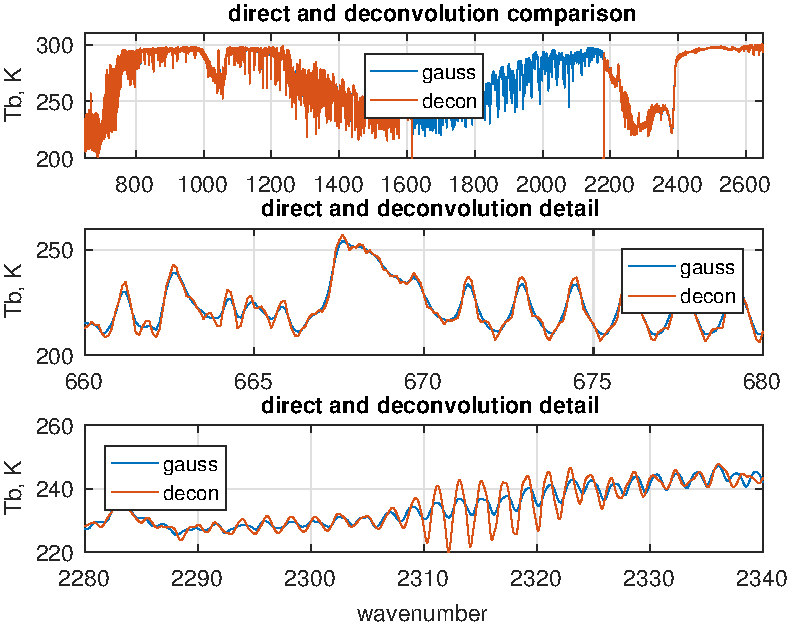
\includegraphics[height=7.5cm]{figures/airs_decon_spec.pdf}
  \caption{spectra from fitting profile 1 for the L1c deconvolution
    and direct convolution to the $0.1$~\wn\ intermediate grid with
    an oversampled resolving power of 2000}
  \label{dspec}
\end{figure}

\begin{figure} % source decon_test1.m
  \centering
  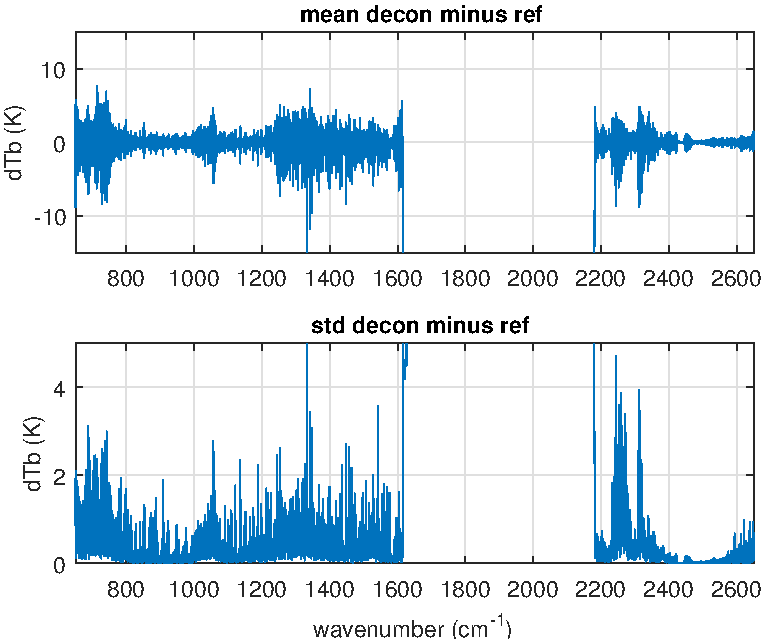
\includegraphics[height=7.5cm]{figures/airs_decon_diff.pdf}
  \caption{mean and standard deviation over the 49 fitting profiles
    for the L1c deconvolution minus direct convolution to the
    $0.1$~\wn\ intermediate grid with an oversampled resolving
    power of 2000}
  \label{ddiff}
\end{figure}

\begin{figure} % source L1d_test2.m
  \centering
  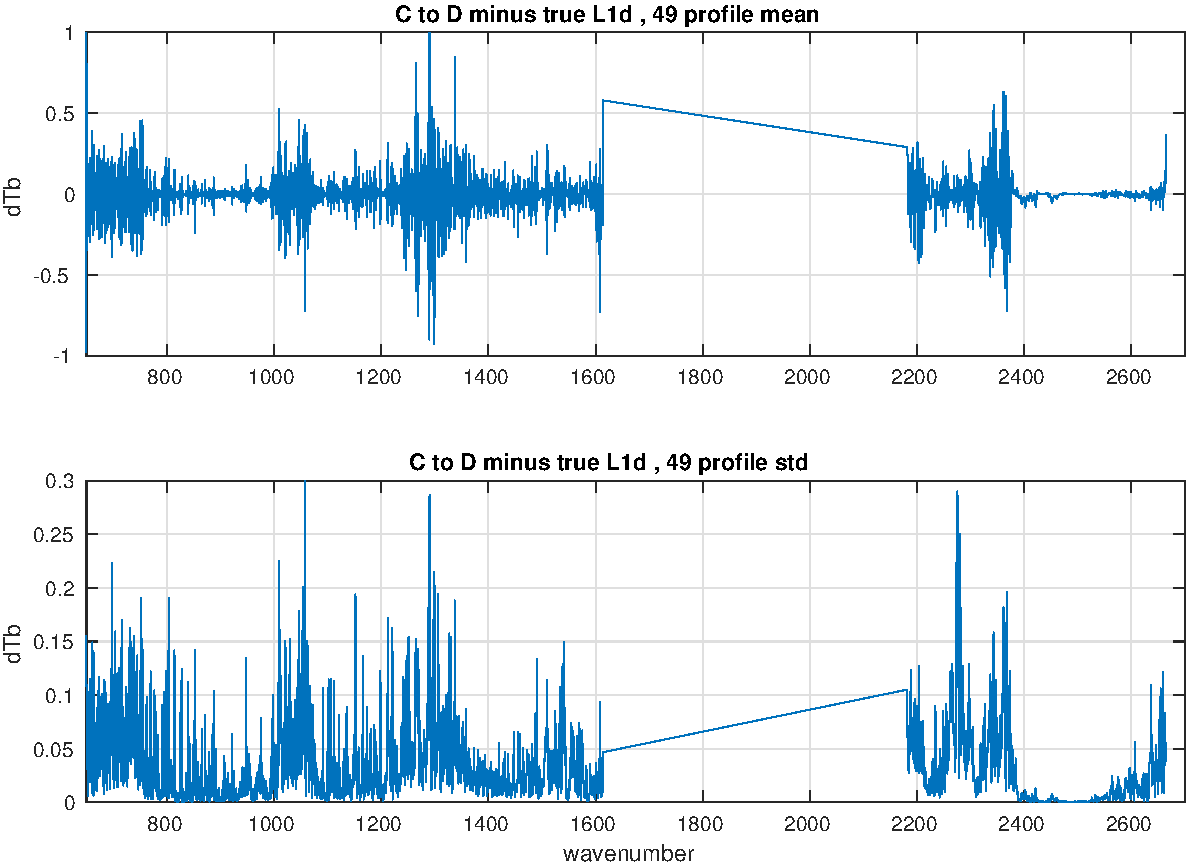
\includegraphics[height=7.5cm]{figures/CtoD1200_diff.pdf}
  \caption{mean and standard deviation over the 49 fitting profiles
    for the L1c deconvolution minus reconvolution to an L1d basis
    with $v_0=649.622$~\wn and a resolving power of 1200}
  \label{L1d1200}
\end{figure}

\begin{figure} % source L1d_test2.m
  \centering
  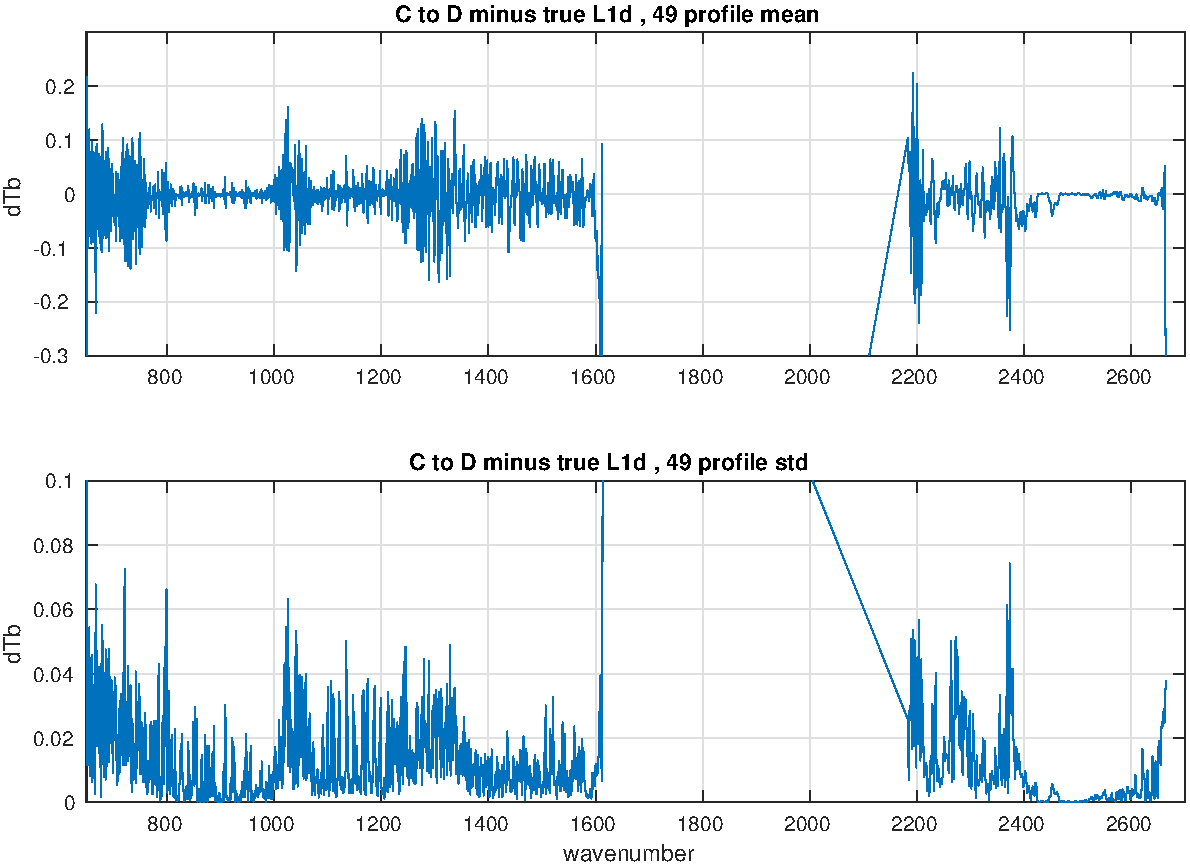
\includegraphics[height=7.5cm]{figures/CtoD700s_diff.pdf}
  \caption{mean and standard deviation over the 49 fitting profiles
    for the L1c deconvolution minus reconvolution to an L1d basis
    with $v_0=649.822$~\wn\ and a resolving power of 700}
  \label{L1d700s}
\end{figure}

\begin{figure} % source L1d_test2.m
  \centering
  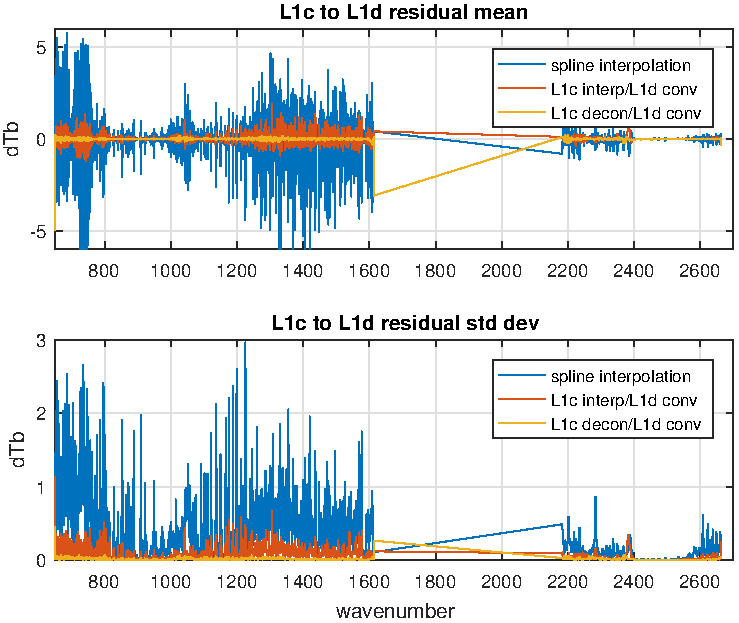
\includegraphics[height=7.5cm]{figures/CtoD_interp_diff.pdf}
  \caption{spline interpolation, interpolation with convolution, 
    and deconvolution with convolution for the {\airs} L1c to L1d
    translation with $v_0=649.822$~\wn\ and a resolving power of 700}
  \label{interpL1d}
\end{figure}

\FloatBarrier
\section{AIRS to CrIS translation}
\label{airs2cris}

For the {\cris} standard resolution mode the channel spacing is
$0.625$ {\wn} for the LW, 1.25~{\wn} for the MW, and 2.5~{\wn} for
the SW bands.  The first step in the {\airs} L1c to {\cris}
translation is to deconvolve the {\airs} channel radiances to the
0.1~{\wn} intermediate grid, the nominal {\airs} SRF resolution.
Then for each {\cris} band, we

\begin{itemize}
  \item find the {\airs} and {\cris} band intersection

  \item apply a bandpass filter to the deconvolved {\airs} radiances
    to restrict them to the intersection, with a rolloff outside the
    intersection

  \item reconvolve the filtered spectra to the {\cris} user grid

\end{itemize}

Translations are validated by comparison with calculated reference
truth.  For the results presented in this section we start with 49
fitting profiles spanning a significant range of atmospheric
conditions \cite{sarta1,sarta2}.  Upwelling radiance is calculated
at a 0.0025 {\wn} grid with kcarta \cite{kcarta1} over a band
spanning the {\airs} and {\cris} response functions.  ``True
{\airs}'' is calculated by convolving the kcarta radiances with
{\airs} SRFs, and ``true {\cris}'' by convolving kcarta radiances to
a sinc basis at the {\cris} user-grid specifications.  {\airs} is
then translated to {\cris} to get ``{\airs} {\cris}'', and this is
compared with true {\cris}.  This validation assumes perfect
knowledge of the {\airs} and {\cris} instrument response functions
and so gives only a lower bound on residuals, and on how well the
translations can work in practice.  The better we know the response
functions, the closer real translations can approach these limits.

% Figure \ref{specLW} shows true {\cris}, true {\airs}, deconvolved
% {\airs}, and {\airs} {\cris}.  In the first subplot we mainly see
% the greater fine structure in the deconvolution.  The second subplot
% shows details from 660 to 680 {\wn}.  

Figures \ref{diffLW}, \ref{diffMW}, and \ref{diffSW} show the mean
and standard deviation of true {\cris} minus {\airs} {\cris} for the
49 fitting profiles, with and without Hamming apodization, for each
of the {\cris} bands.  Figures \ref{meanAll} and \ref{stdAll}
summarize the mean and standard deviation of the residuals for
Hamming apodized radiances.  The residual has a high frequency
component with a period of 2 channel steps that is significantly
reduced by the apodization.  The constant or DC bias (the mean of
the residuals over frequency) is very close to zero for the apodized
residuals: $0.002$~K for the LW, $-0.005$~K for the MW, and
$0.001$~K for the SW.

% \begin{figure} % source a2cris_test1
%   \centering
%   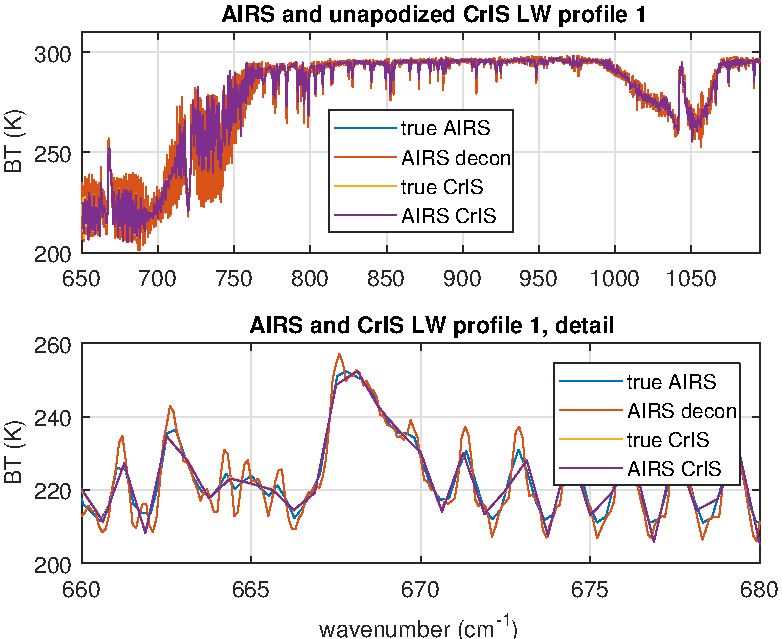
\includegraphics[height=7.5cm]{figures/a2cris_spec_LW.pdf}
%   \caption{true {\cris}, true {\airs}, deconvolved {\airs}, and
%     {\airs} {\cris}}
%   \label{specLW}
% \end{figure}

\begin{figure} % source a2cris_test1
  \centering
  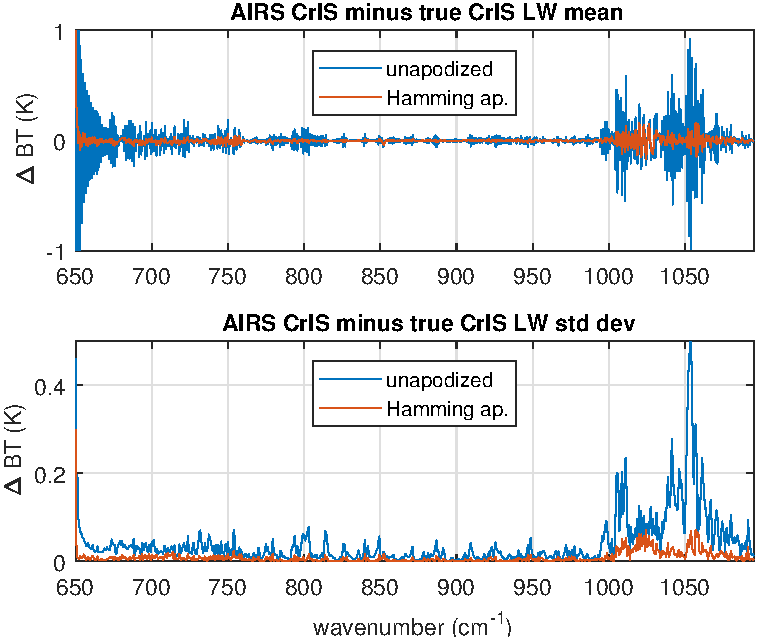
\includegraphics[height=7.5cm]{figures/a2cris_diff_LW.pdf}
  \caption{Mean and standard deviation of unapodized and Hamming
    apodized {\airs} {\cris} minus true {\cris}, for the {\cris} LW
    band}
  \label{diffLW}
\end{figure}

\begin{figure} % source a2cris_test1
  \centering
  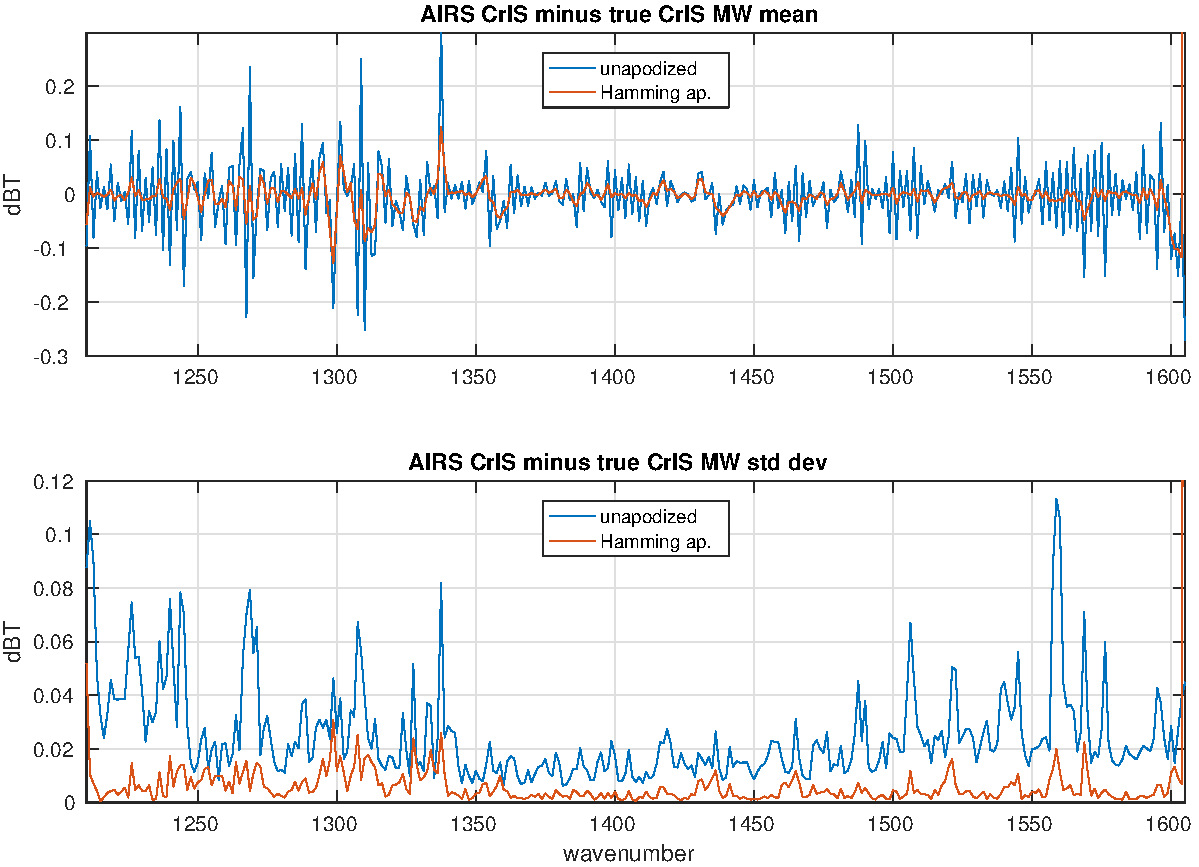
\includegraphics[height=7.5cm]{figures/a2cris_diff_MW.pdf}
  \caption{Mean and standard deviation of unapodized and Hamming
    apodized {\airs} {\cris} minus true {\cris}, for the {\cris} MW
    band}
  \label{diffMW}
\end{figure}

\begin{figure} % source a2cris_test1
  \centering
  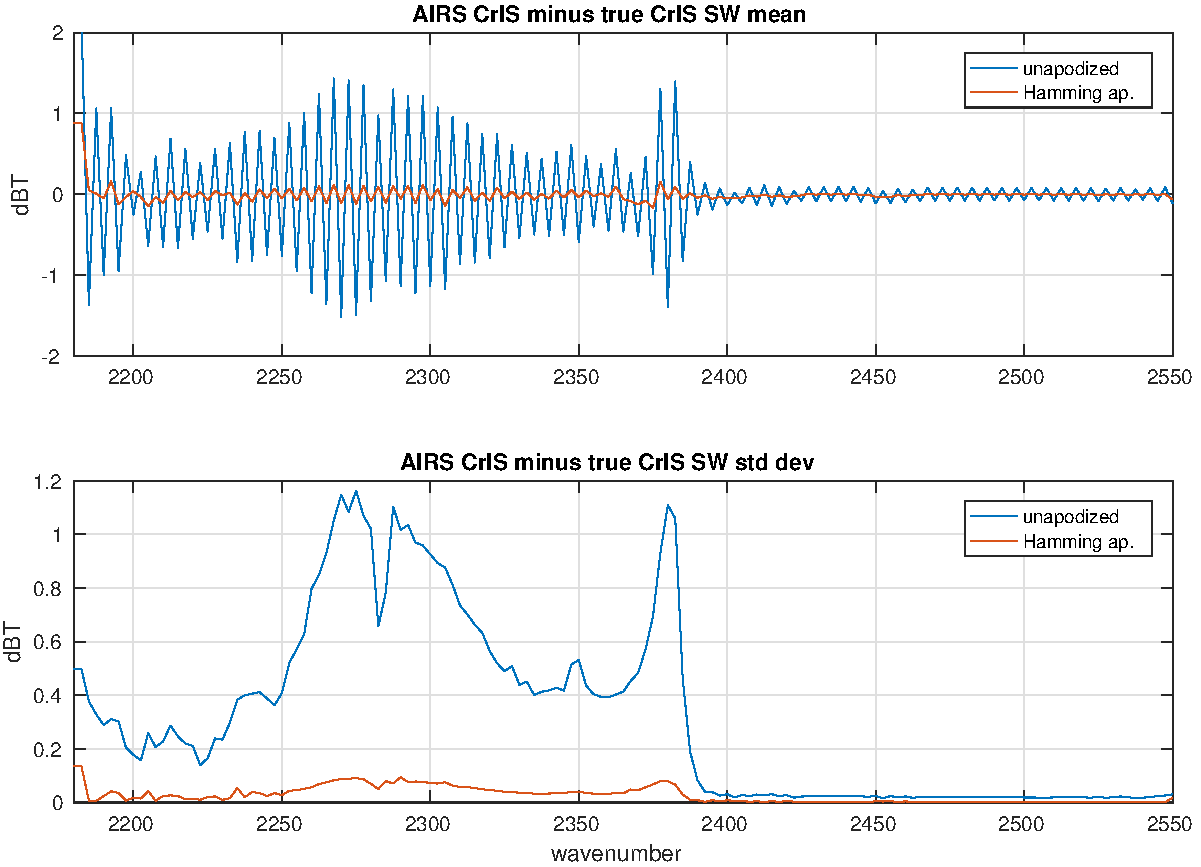
\includegraphics[height=7.5cm]{figures/a2cris_diff_SW.pdf}
  \caption{Mean and standard deviation of unapodized and Hamming
    apodized {\airs} {\cris} minus true {\cris}, for the {\cris} SW
    band}
  \label{diffSW}
\end{figure}

\begin{figure} % source a2cris_plot1.m
  \centering
  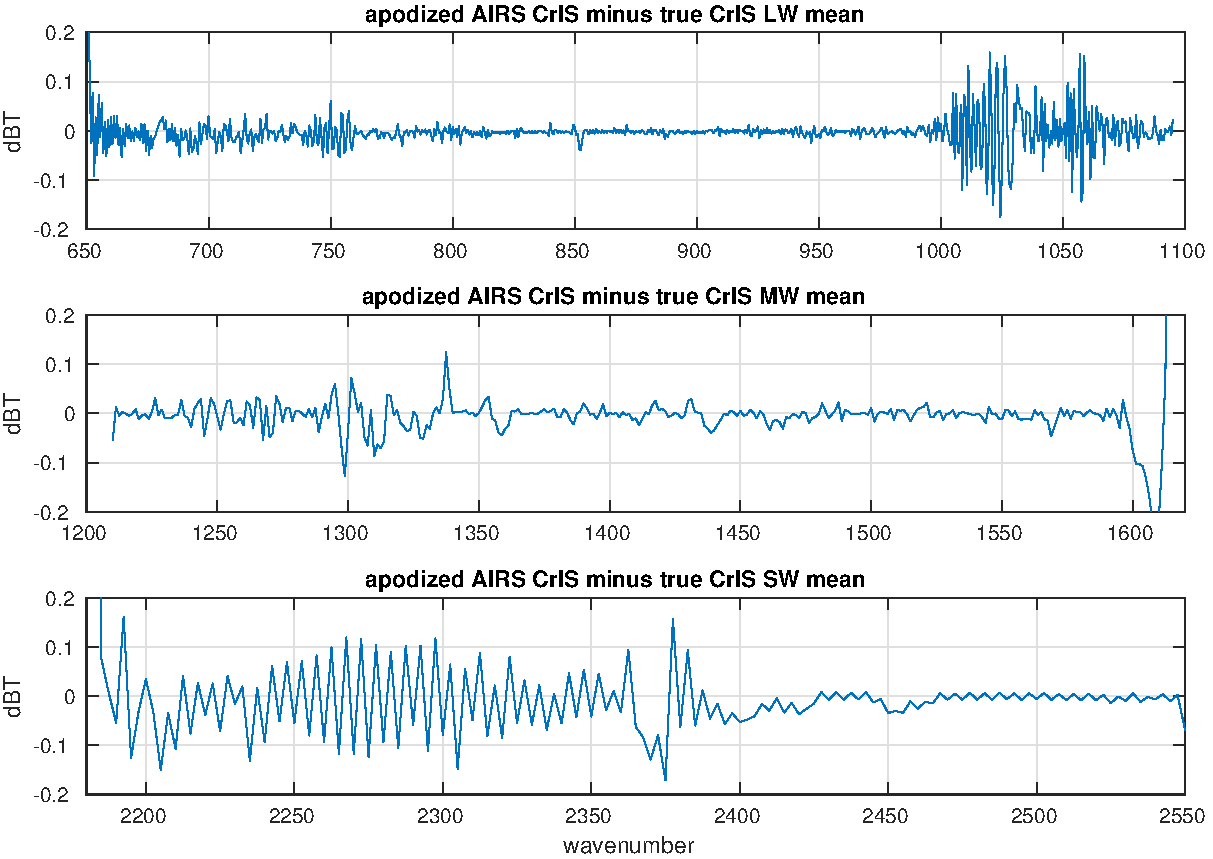
\includegraphics[height=7.5cm]{figures/combo_ap_dif_mean.pdf}
  \caption{Mean of apodized residuals for all three {\cris} bands}
  \label{meanAll}
\end{figure}

\begin{figure} % source a2cris_plot1.m
  \centering
  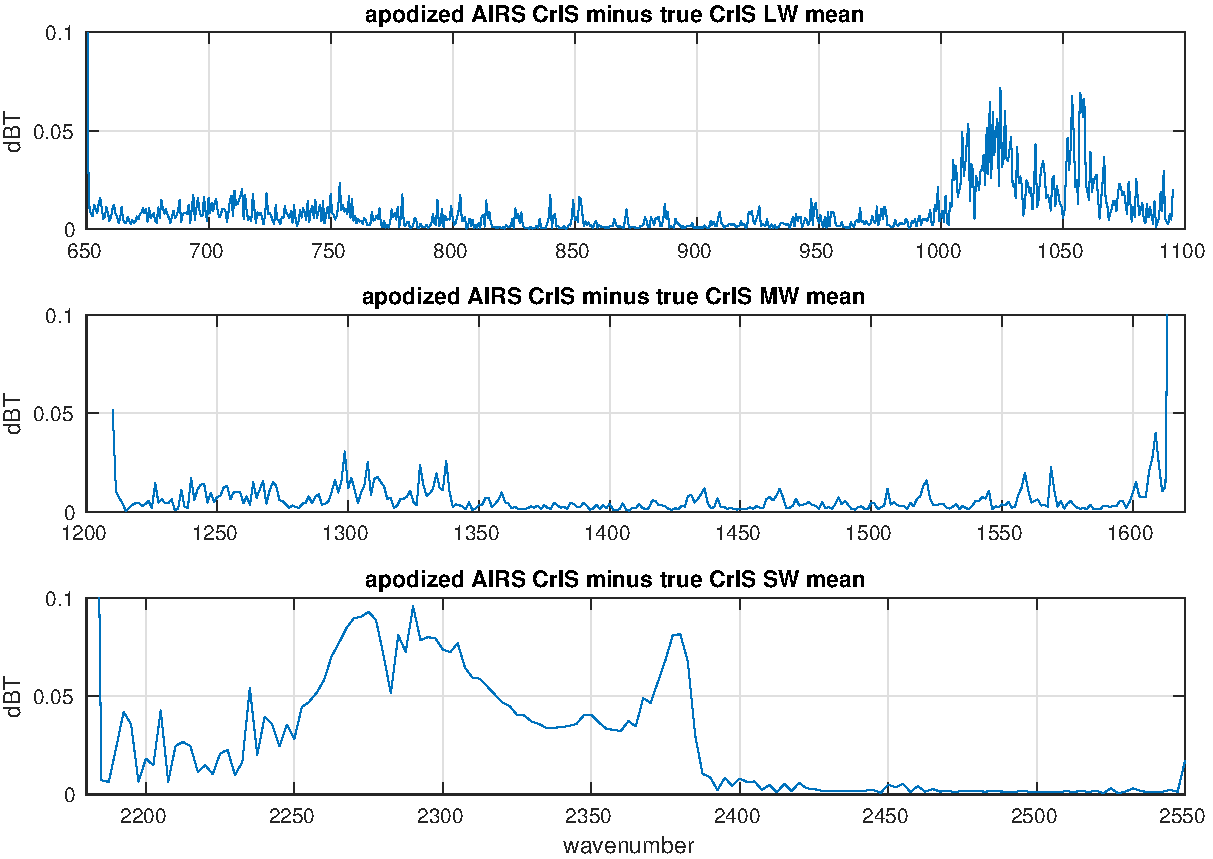
\includegraphics[height=7.5cm]{figures/combo_ap_dif_std.pdf}
  \caption{Standard deviation of apodized residuals for all three
    {\cris} bands}
  \label{stdAll}
\end{figure}

\begin{figure} % source a2cris_test1
  \centering
  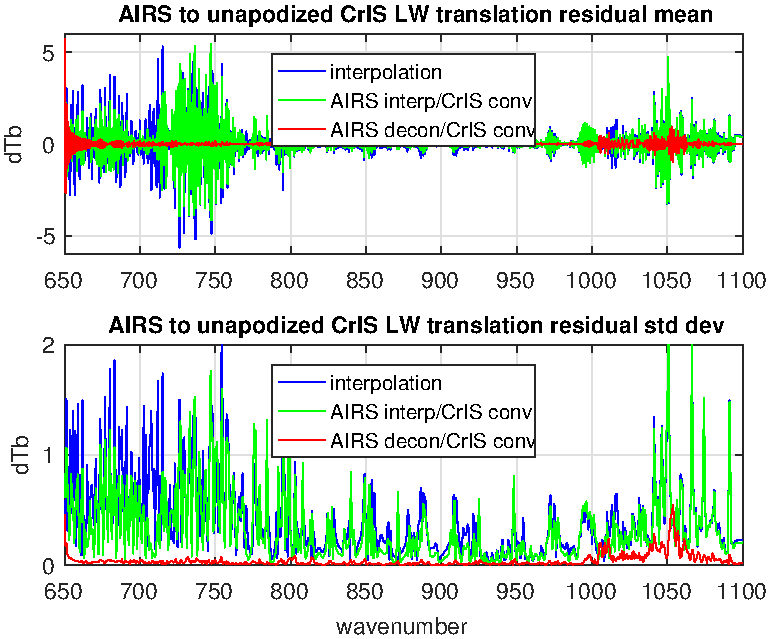
\includegraphics[height=7.5cm]{figures/a2cris_interp_LW.pdf}
  \caption{spline interpolation, interpolation with convolution, 
    and deconvolution with convolution for the {\cris} LW band}
  \label{intpLW}
\end{figure}

Deconvolution is significantly better than interpolation for the
{\airs} to {\cris} translation.  We consider two cases.  For the
first, start with true {\airs} and interpolate radiances directly 
to the {\cris} user grid with a cubic spline.  For the second,
interpolate true {\airs} to the 0.1 {\wn} intermediate grid with a
cubic spline and then convolve this to the use {\cris} user grid.
Figure~\ref{intpLW} shows interpolated {\cris} minus true {\cris}
for the LW band, without apodization.  The two-step interpolation
works a little better than the simple spline, but both residuals are
significantly larger than for the translation with deconvolution.
Results for the MW are similar, while the unapodized comparison is
less clear for the SW.  With Hamming apodization, the residuals with
deconvolution are significantly less than interpolation for all
three bands.

\FloatBarrier
\section{Statisitcal Refinement}
\label{statfix}

Residuals for the {\airs} to apodized {\cris} translation are
already small, and have no significant DC bias.  But there is some
regularity in the residual, including an oscillation with period two
channel steps.  We show that a linear correction can significantly
reduce this residual.  This is a standard technique but worth
describing briefly because the reduction is significant.

For these tests we start with kcarta radiances calculated from a 
set of 7377 radiances calculated from mostly cloudy AIRS profiles.
spanning several consecutive days.  These are split randomly into
dependent and independent sets.  Bias or regression coefficients are
taken from the dependent set, and tests are done on the independent
set.  As with the 49 profile set ``true {\airs}'' channel radiances
are calculated by convolving with {\airs} SRFs and ``true {\cris}''
by convolving to the {\cris} instrument specifications.

Note the difference in statistical approaches here and in section
\ref{airs2cris}.  There we used a small, largely uncorrelated set of
49 profiles chosen to span all common clear atmospheric conditions,
and intended for developing and testing radiative transfer codes.
For the statistical correction we use a more typical mix of clear
and cloudy data spanning several days, moderately correlated, and
large enough to allow for partition into significant dependent and
independent sets.

Figure \ref{statLW} is a comparison of bias, linear, and quadratic
corrections for a representative dependend/independent partition.
The residuals vary with the partition but the standard deviation is
consistently significantly less for the linear and quadratic cases.
The linear and quadratic corrections are nearly identical, the
quadratic coefficient is very close to zero.  Figure \ref{coefLW}
shows the weights for the linear fits shown above.  The $a$ weight
is very close to 1 and the $b$ weight to earlier bias values.

Figures \ref{statMW} and \ref{statSW} show the linear correction 
is giving a similar significant improvement in the MW standard
deviation in comparison with the LW, and a small improvement in the
SW.  As in the LW the mean residuals vary significantly depending on
the dependent/independent partition, but the standard deviations are
relatively stable.

\begin{figure} % source a2cris_stat4.m
  \centering
  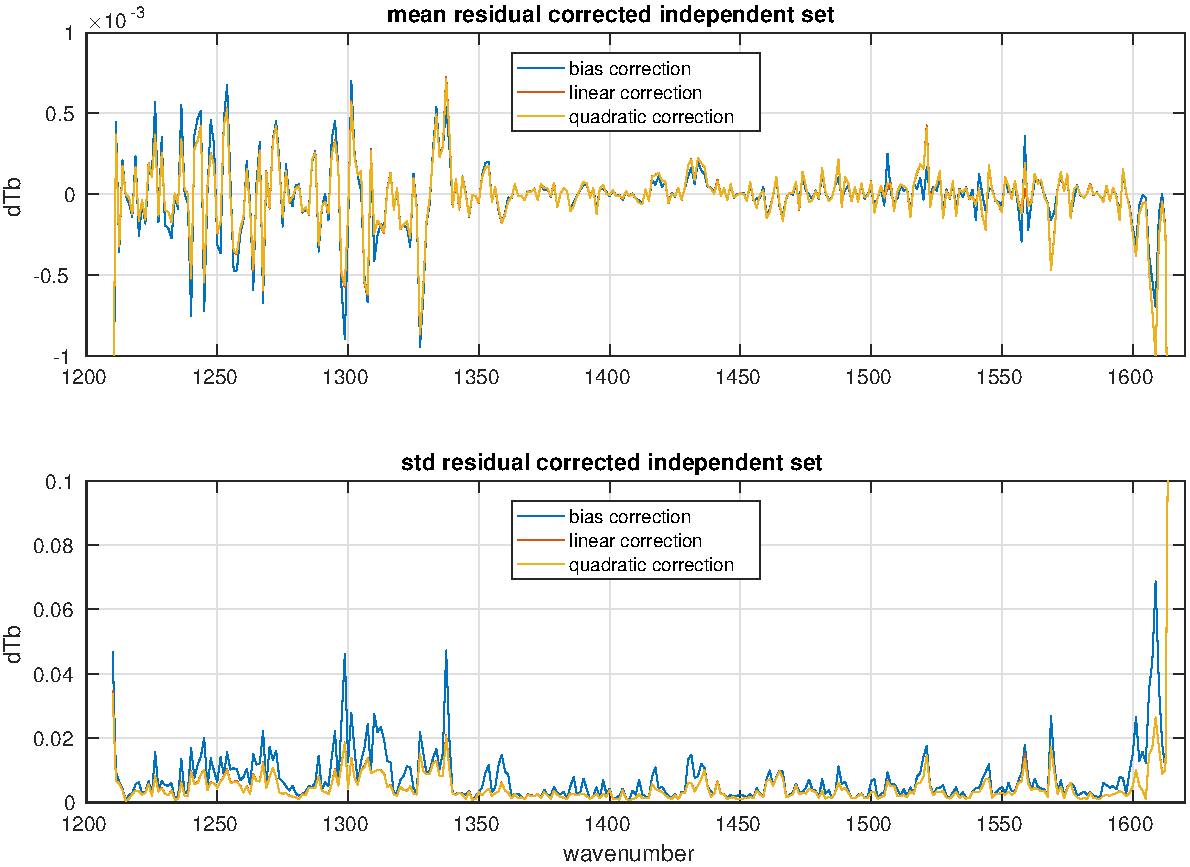
\includegraphics[height=7.5cm]{figures/a2cris_stat_LW.pdf}
  \caption{Mean and standard deviation of LW corrected apodized
    residuals for the independent subset of the 7377 profile set}
  \label{statLW}
\end{figure}

\begin{figure} % source a2cris_stat4.m
  \centering
  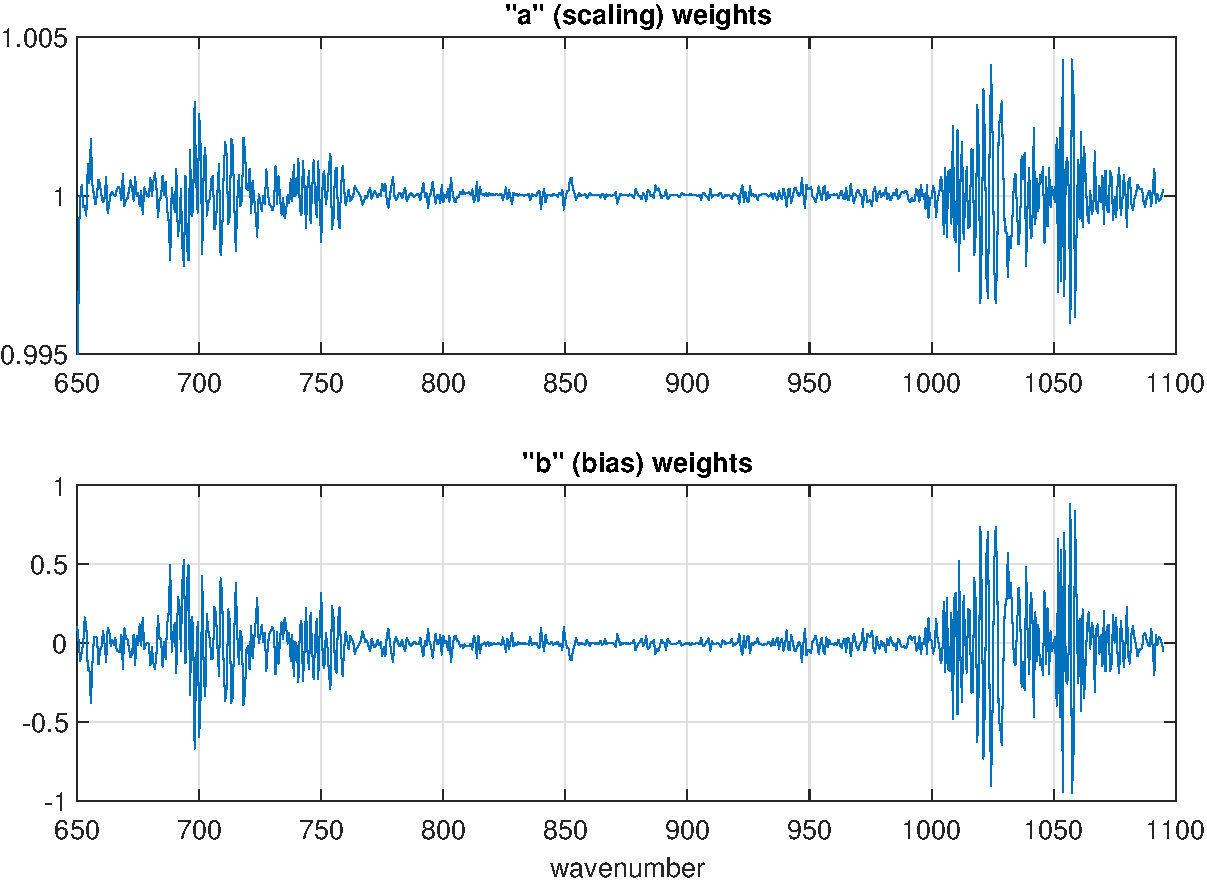
\includegraphics[height=7.5cm]{figures/a2cris_coef_LW.pdf}
  \caption{LW $a$ and $b$ weights for the linear correction $ax+b$}
  \label{coefLW}
\end{figure}

\begin{figure} % source a2cris_stat4.m
  \centering
  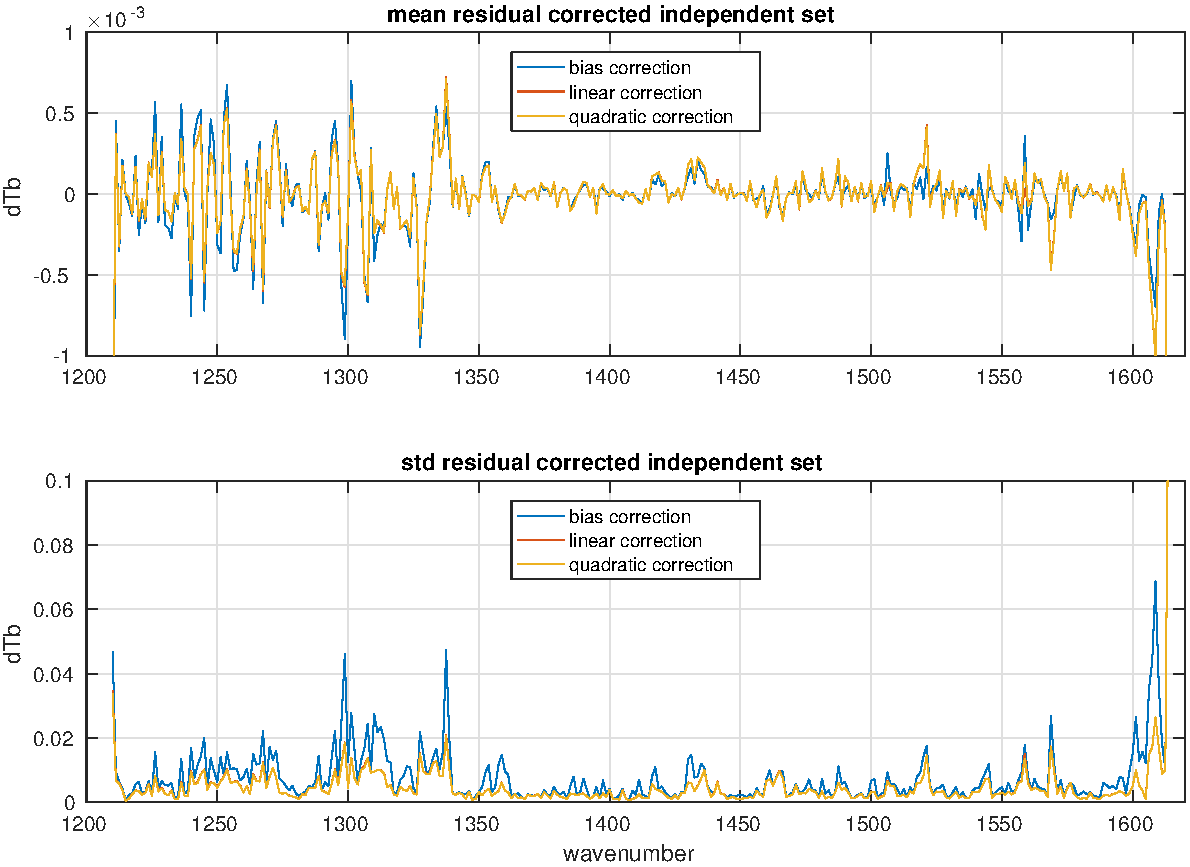
\includegraphics[height=7.5cm]{figures/a2cris_stat_MW.pdf}
  \caption{Mean and standard deviation of MW corrected apodized
    residuals for the independent subset of the 7377 profile set}
  \label{statMW}
\end{figure}

\begin{figure} % source a2cris_stat4.m
  \centering
  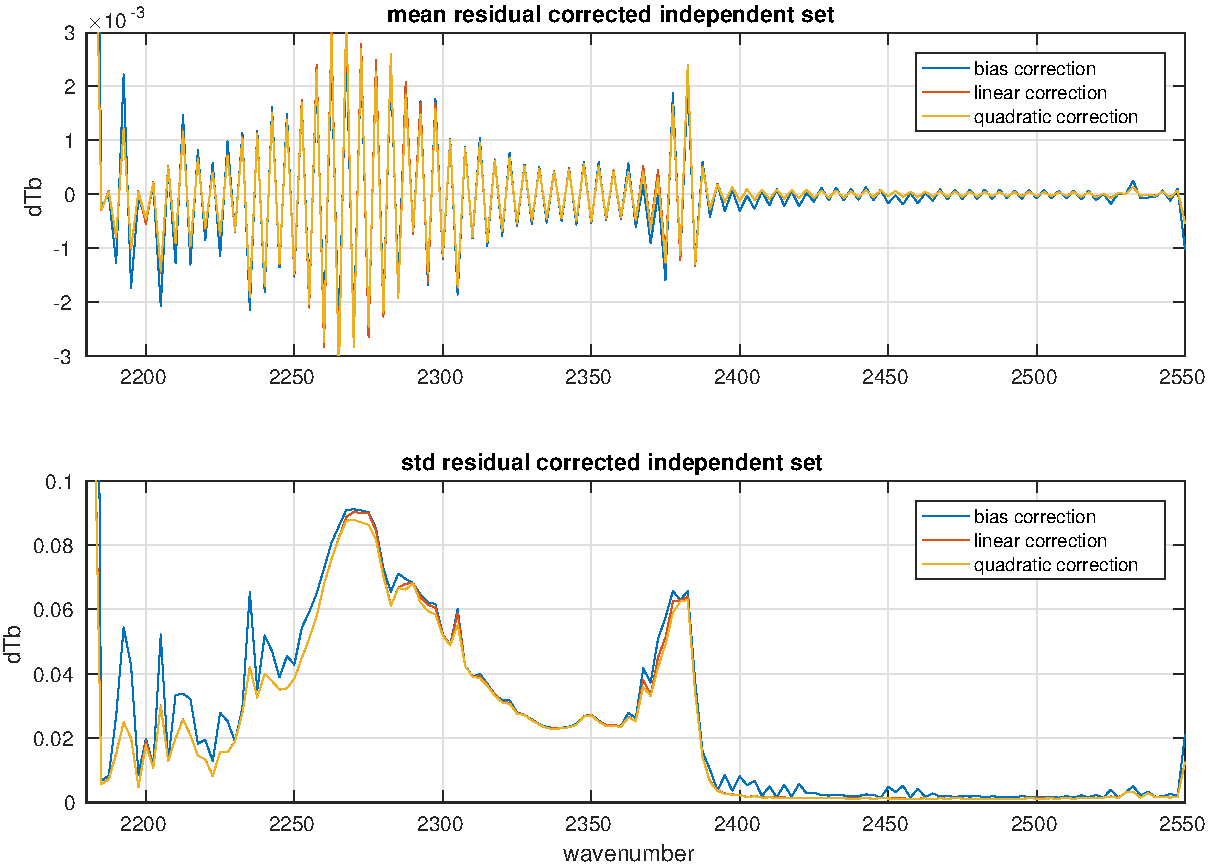
\includegraphics[height=7.5cm]{figures/a2cris_stat_SW.pdf}
  \caption{Mean and standard deviation of SW corrected apodized
    residuals for the independent subset of the 7377 profile set}
  \label{statSW}
\end{figure}

% \FloatBarrier
% \section{Deconvolution to constant resolving power}
% \label{airsL1d}
% 
% Section \ref{decon} raised the question of the inherent resolution
% of the deconvolution.  There we compared the deconvolution (without
% reconvolution) to calculated radiances with an oversampled resolving
% power of 2000.  But the residual was quite large.  
% 
% Similar to the situation with convolution to the {\cris} user grid,
% 

\FloatBarrier
\section{Applications and conclusions}
\label{appcon}

\FloatBarrier
\bibliographystyle{abbrv}
\bibliography{decon}

\end{document}

